\documentclass{article}%
\usepackage[T1]{fontenc}%
\usepackage[utf8]{inputenc}%
\usepackage{lmodern}%
\usepackage{textcomp}%
\usepackage{lastpage}%
\usepackage[head=40pt,margin=0.5in,bottom=0.6in]{geometry}%
\usepackage{graphicx}%
%
\title{\textbf{Trabajadores de la Cancillería protestaron por bajos sueldos y en rechazo al pago en petros}}%
\author{CRISBEL VARELA}%
\date{20/11/2018}%
%
\begin{document}%
\normalsize%
\maketitle%
\textbf{URL: }%
http://www.eluniversal.com/politica/26289/trabajadores{-}de{-}la{-}cancilleria{-}protestan{-}por{-}bajos{-}sueldos{-}y{-}en{-}rechazo{-}a{-}las{-}tablas{-}salariales\newline%
%
\textbf{Periodico: }%
EU, %
ID: %
26289, %
Seccion: %
politica\newline%
%
\textbf{Palabras Claves: }%
NO\_TIENE\newline%
%
\textbf{Derecho: }%
2.3, %
Otros Derechos: %
, %
Sub Derechos: %
2.3.4\newline%
%
\textbf{EP: }%
SI\newline%
\newline%
%
\textbf{\textit{Los empleados del Ministerio de Relaciones Exteriores también manifestaron su descontento por la unificación de tablas salariales}}%
\newline%
\newline%
%
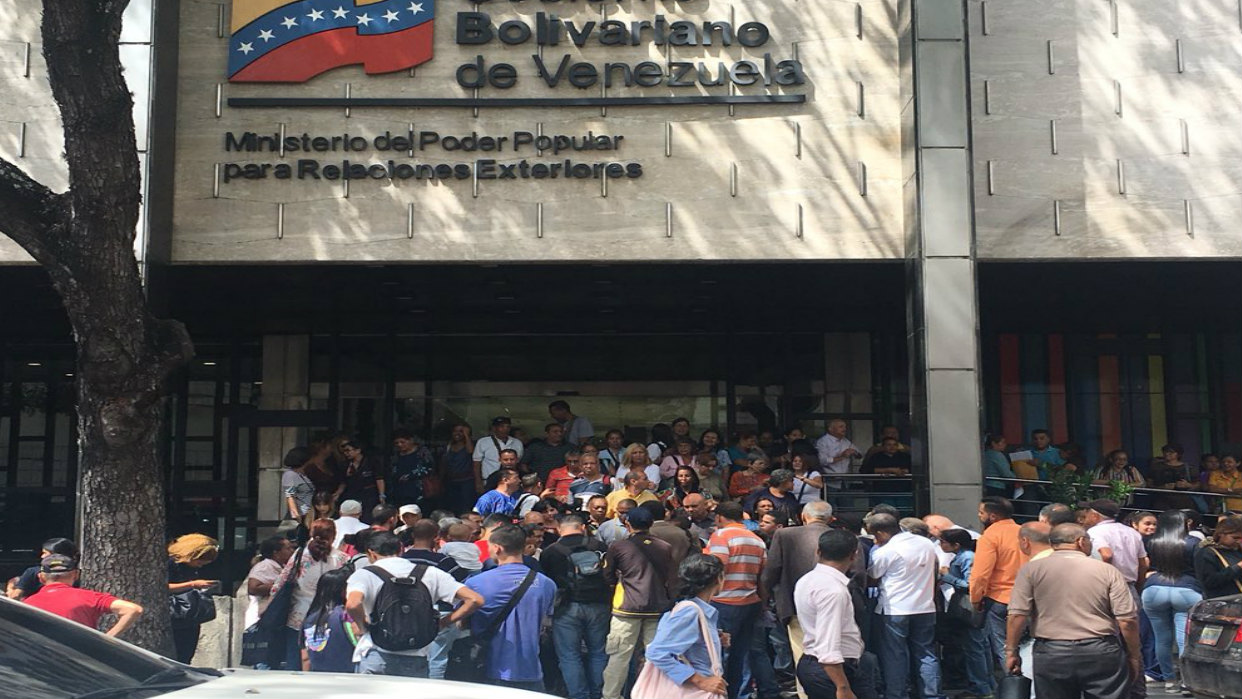
\includegraphics[width=300px]{206.jpg}%
\newline%
%
Caracas.{-} Trabajadores del Ministerio de Relaciones Exteriores protestaron este martes en por los bajos salarios que devengan, la propuesta del Gobierno de realizar el pago de las nóminas en petros y en rechazo a unificación de las tablas salariales.%
\newline%
%
La información la dio a conocer la internacionalista, Giovanna De Michele, a través de la red social Twitter.%
\newline%
%
Desde que entró en vigencia el salario mínimo de 1.800 bolívares soberanos, diversos sectores de la administración pública han protestado en Caracas y el resto del país en rechazo al "irrespeto" de los contratos colectivos.%
\newline%
%
\end{document}